
%% This is file `sample-sigconf-authordraft.tex',
%% generated with the docstrip utility.
%%
%% The original source files were:
%%
%% samples.dtx  (with options: `all,proceedings,bibtex,authordraft')
%% 
%% IMPORTANT NOTICE:
%% 
%% For the copyright see the source file.
%% 
%% Any modified versions of this file must be renamed
%% with new filenames distinct from sample-sigconf-authordraft.tex.
%% 
%% For distribution of the original source see the terms
%% for copying and modification in the file samples.dtx.
%% 
%% This generated file may be distributed as long as the
%% original source files, as listed above, are part of the
%% same distribution. (The sources need not necessarily be
%% in the same archive or directory.)
%%
%%
%% Commands for TeXCount
%TC:macro \cite [option:text,text]
%TC:macro \citep [option:text,text]
%TC:macro \citet [option:text,text]
%TC:envir table 0 1
%TC:envir table* 0 1
%TC:envir tabular [ignore] word
%TC:envir displaymath 0 word
%TC:envir math 0 word
%TC:envir comment 0 0
%%
%% The first command in your LaTeX source must be the \documentclass
%% command.
%%
%% For submission and review of your manuscript please change the
%% command to \documentclass[manuscript, screen, review]{acmart}.
%%
%% When submitting camera ready or to TAPS, please change the command
%% to \documentclass[sigconf]{acmart} or whichever template is required
%% for your publication.
%%
%%


\documentclass[sigconf,authordraft]{acmart}

%%
%% \BibTeX command to typeset BibTeX logo in the docs
\AtBeginDocument{%
  \providecommand\BibTeX{{%
    Bib\TeX}}}

%% Rights management information.  This information is sent to you
%% when you complete the rights form.  These commands have SAMPLE
%% values in them; it is your responsibility as an author to replace
%% the commands and values with those provided to you when you
%% complete the rights form.
%%\setcopyright{acmlicensed}
%%\copyrightyear{2018}
%%\acmYear{2018}
%%\acmDOI{XXXXXXX.XXXXXXX}
%% These commands are for a PROCEEDINGS abstract or paper.
\acmConference[Conference acronym 'WISSA]{Wissenschaftliches Arbeiten}{February 04,
  2025}{Dresden, SN}
%%
%%  Uncomment \acmBooktitle if the title of the proceedings is different
%%  from ``Proceedings of ...''!
%%
%%\acmBooktitle{Woodstock '18: ACM Symposium on Neural Gaze Detection,
%%  June 03--05, 2018, Woodstock, NY}
%%\acmISBN{978-1-4503-XXXX-X/18/06}


%%
%% Submission ID.
%% Use this when submitting an article to a sponsored event. You'll
%% receive a unique submission ID from the organizers
%% of the event, and this ID should be used as the parameter to this command.
%%\acmSubmissionID{123-A56-BU3}

%%
%% For managing citations, it is recommended to use bibliography
%% files in BibTeX format.
%%
%% You can then either use BibTeX with the ACM-Reference-Format style,
%% or BibLaTeX with the acmnumeric or acmauthoryear sytles, that include
%% support for advanced citation of software artefact from the
%% biblatex-software package, also separately available on CTAN.
%%
%% Look at the sample-*-biblatex.tex files for templates showcasing
%% the biblatex styles.
%%

%%
%% The majority of ACM publications use numbered citations and
%% references.  The command \citestyle{authoryear} switches to the
%% "author year" style.
%%
%% If you are preparing content for an event
%% sponsored by ACM SIGGRAPH, you must use the "author year" style of
%% citations and references.
%% Uncommenting
%% the next command will enable that style.
%%\citestyle{acmauthoryear}
%%
%% end of the preamble, start of the body of the document source.

%% EDIT VON PAUL
\usepackage{tabularx}
\usepackage{graphicx} % Für Bilder
\usepackage[ngerman]{babel}
\newcommand{\anf}[1]{\glqq{}#1\grqq{}}  % Anführungszeichen

\begin{document}



%%
%% The "title" command has an optional parameter,
%% allowing the author to define a "short title" to be used in page headers.
\title{Auswirkungen von Quantencomputern auf aktuelle Verschlüsselungsalgorithmen}

%%
%% The "author" command and its associated commands are used to define
%% the authors and their affiliations.
%% Of note is the shared affiliation of the first two authors, and the
%% "authornote" and "authornotemark" commands
%% used to denote shared contribution to the research.
\author{Daniel Josef Heinrich Haus}
\email{s3005733@ba-sachsen.de}
\affiliation{
  \institution{DHSN}
  \city{Dresden}
  \state{Sachsen}
  \country{Deutschland}
}
\author{Ben Kaiser}
\email{s3005541@ba-sachsen.de}
\affiliation{
  \institution{DHSN}
  \city{Dresden}
  \state{Sachsen}
  \country{Deutschland}
}
\author{Paul Zenker}
\email{s3005664@ba-sachsen.de}
\affiliation{
  \institution{DHSN}
  \city{Dresden}
  \state{Sachsen}
  \country{Deutschland}
}
\author{Felix Brockwitz}
\email{s3005540@ba-sachsen.de}
\affiliation{
  \institution{DHSN}
  \city{Dresden}
  \state{Sachsen}
  \country{Deutschland}
}
\author{Matheo Zoeke}
\email{s3005785@ba-sachsen.de}
\affiliation{
  \institution{DHSN}
  \city{Dresden}
  \state{Sachsen}
  \country{Deutschland}
}

%%
%% By default, the full list of authors will be used in the page
%% headers. Often, this list is too long, and will overlap
%% other information printed in the page headers. This command allows
%% the author to define a more concise list
%% of authors' names for this purpose.
\renewcommand{\shortauthors}{DJHH, BK, PZ, FB, MZ}

%%
%% The abstract is a short summary of the work to be presented in the
%% article.

%%
%% The code below is generated by the tool at http://dl.acm.org/ccs.cfm.
%% Please copy and paste the code instead of the example below.
%%
\begin{CCSXML}
  <ccs2012>
     <concept>
         <concept_id>10002978.10002979.10002984</concept_id>
         <concept_desc>Security and privacy~Information-theoretic techniques</concept_desc>
         <concept_significance>500</concept_significance>
         </concept>
   </ccs2012>
\end{CCSXML}
  
\ccsdesc[500]{Security and privacy~Information-theoretic techniques}

%%
%% Keywords. The author(s) should pick words that accurately describe
%% the work being presented. Separate the keywords with commas.
\keywords{Security, Cryptography, RSA, Shor´s Algorithm, AES, Quantum Computers}
%% A "teaser" image appears between the author and affiliation
%% information and the body of the document, and typically spans the
%% page.
\begin{teaserfigure}
  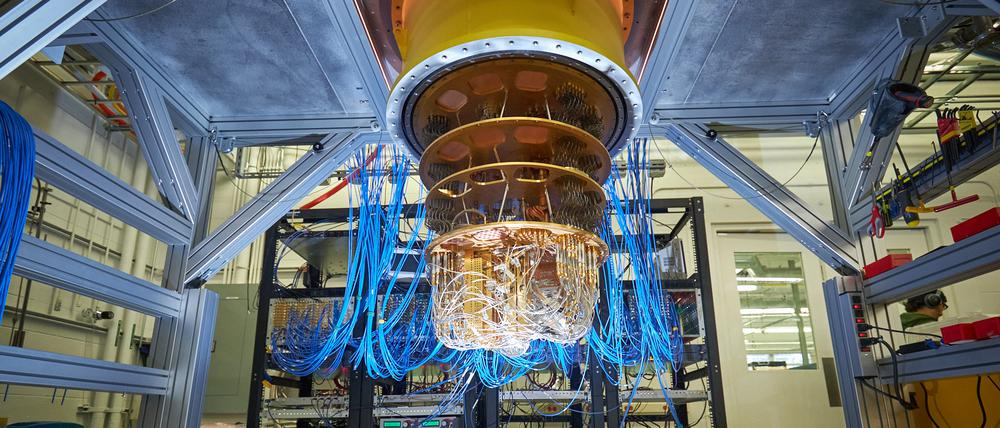
\includegraphics[width=\textwidth]{sampleteaser}
  \caption{Google Quantum AI, 2019.\cite{teaserfigure}}
  \Description{Berichtigter Quantencomputer: Neuartiger Chip korrigiert viele seiner Fehler}
  \label{fig:teaser}
\end{teaserfigure} 


%%
%% This command processes the author and affiliation and title
%% information and builds the first part of the formatted document.
\maketitle
\section*{Abstract}
  Die fortschreitende Entwicklung von Quantencomputern stellt eine erhebliche Bedrohung 
  für die Sicherheit moderner Verschlüsselungssysteme dar. Dieser Beitrag untersucht die 
  Auswirkungen von Quantencomputern auf symmetrische und asymmetrische Verschlüsselungsalgorithmen, 
  mit besonderem Fokus auf RSA und AES. Im Mittelpunkt stehen die Herausforderungen, die 
  durch Algorithmen wie Shor’s Algorithmus und die Quanten-Fourier-Transformation entstehen.
  Während RSA als asymmetrisches Verfahren durch die Zerlegung großer Zahlen in ihre 
  Primfaktoren auf Basis der klassischen Rechenleistung gesichert ist, zeigt Shor’s Algorithmus, 
  dass Quantencomputer diese Aufgabe effizient lösen können, wodurch die Sicherheit von RSA 
  vollständig untergraben wird. Der Beitrag erklärt detailliert die Funktionsweise von Shor’s Algorithmus, der auf der 
  Quanten-Fourier-Transformation basiert, und zeigt auf, wie diese Technologie es ermöglicht, 
  die periodischen Eigenschaften von Zahlen effizient zu berechnen. Zudem wird die allgemeine 
  Bedeutung der Kryptografie im digitalen Zeitalter beleuchtet.

\newpage
\section{Einleitung}
Forschungsfrage 1: 
Was sind die Auswirkungen von Quantencomputern auf 
aktuelle symmetrische und asymmetrische Verschlüsselungsalgorithmen 
am Beispiel von RSA und AES?

Forschungsfrage 2: 
Wie beeinflusst die Entwicklung von Quantencomputern die langfristige 
Sicherheit von Daten, und welche Strategien können Organisationen 
implementieren, um "Store-now, decrypt-later"-Angriffe zu verhindern?
\section{Quantencomputer Allgemein}
\label{sec:quantencomputer}
Der Unterschied zwischen einem Quantencomputer und einem normalen Computer ist die Verwendung von Quantenbits \cite{quantencomputer_2024} anstelle der üblichen Bits, womit ein Zweistandsystem \cite{zweizustandssystem_nodate} erstellt wird, wobei ein Qubit entweder einer 1 oder einer 0 entspricht und das System aus mindestens zwei Bits besteht. Damit können verschiedene Werte erstellt werden, wie 1;1, 0;1, 0;0, 1;0, wie in normalen Transistoren.

Der Unterschied zu konventionellen Computern ist nun, dass zwei Qubits, solange keine Messungen des gesamten Systems stattfinden, aus einer Superposition aus 1 und 0 bestehen. 
Das heißt, dass alle vier Werte des Zweistandsystems parallel zueinander existieren können und es möglich machen, mehrere Berechnungen gleichzeitig durchzuführen.\cite{What_is_quantum_computing_nodate}
Dies wird ermöglicht durch die Quantenverschränkung, wobei zwei Systeme so eng miteinander verbunden sind, dass Wissen über den ersten Teil des Systems mit einer Wahrscheinlichkeitsverteilung ein Wissen über den zweiten gibt, ohne den zweiten Teil gemessen zu haben.\cite{quantenverschrankung_2024}

Ein Qubit könnte zum Beispiel die Polarisationsrichtung eines Photons sein, welches von zwei orthogonalen Richtungen gemessen wird \cite{What_is_quantum_computing_nodate}. 

Hier zählen die sinusförmigen elektromagnetischen Wellen als rechts- 
oder linkszirkular und werden dementsprechend als 1 oder 0 angelegt (Abbildung \ref{fig:elektromagnetische_welle}) \cite{electromagnetic_2024}.

\begin{figure}[h]
    \centering
    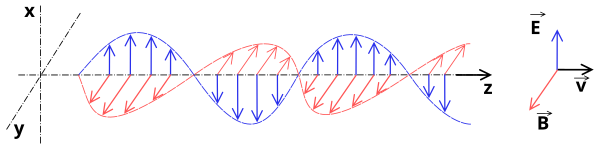
\includegraphics[width=0.45\textwidth]{Onde_electromagnetique.svg.jpg}
    \caption{Eine linear polarisierte elektromagnetische Welle, die in der Z-Achse verläuft.}
    \label{fig:elektromagnetische_welle}
\end{figure}


Andere Implementierungen, ein Zweistandsystem aus Qubits zu erstellen, gibt es auch mit dem Energieniveau von Atomen oder Molekülen bis hin zu Flussrichtungen von Stromkreisen in Supraleitern \cite{supraleitung_nodate}.

Da diese Methoden naturwissenschaftliche Teilchen als Berechnungsbasis nehmen, die von ihrer Größe her kleiner als ein einzelnes Atom sind, spricht man nun von Quantenmechanik. 

Dies führt zu einer der größten Hürden für Quantencomputer, der Dekohärenz, wobei Qubits ihren Quantenzustand durch Umgebungsfaktoren verlieren. Deshalb müssen sie oftmals von außen abgeschirmt und bei Temperaturen nahe dem absoluten Nullpunkt gehalten werden, um den Quantenzustand und somit die Quantenverschränkung aufrechtzuerhalten, die für die Berechnungen nötig sind.

Da die Qubits so sensitiv sind, gibt es auch Schwierigkeiten mit längeren Berechnungen. Oftmals tauchen Fehler in den Qubits auf, die man noch nicht gut genug kompensieren kann. Oft müssen Berechnungen mehrmals durchgeführt werden oder sind in ihrer Länge limitiert.\cite{brubaker_quantum_2024} Es wird weiter an Algorithmen und Systemen geforscht, die sehr vielversprechend sind.

Dies führt zu dem Phänomen  \textit{Store now, decrypt later} was übersetzt heist, jetzt speichern und später entschlüsseln. Zum Beispiel könnten Daten, die mit RSA verschlüsselt werden und heute noch sicher sind, durch die deutlich schnellere Berechnung von Primzahlen durch Quantencomputer in der Zukunft sehr viel leichter entschlüsselt werden. 
Informationen, die heute als sensibel gelten, sind es auch noch in Zukunft, was bedeutet, dass es notwendig ist, heute schon Alternativen für Verschlüsselungen zu verwenden, die gegen leistungsfähigere Quantencomputer gesichert sind.\cite{veritasium_how_2023}

Andere Anwendungsbereiche für Quantencomputer gibt es in der Medizin, 
Materialwissenschaften, Finanzmodellierung 
und Verkehrsoptimierung. \cite{Applications_10_nodate}



\section{Kryptografie\textendash Grundlagen}
Verschlüsselungsalgorithmen werden grundlegend in zwei Gruppen unterteilt.
Die erste Gruppe ist symmetrische Verschlüsselung, welche Grundlegend zum Verschlüsseln von Daten
oder Texten verwendet wird. Diese verwendet zum Ver\textendash\ und Entschlüssen den gleichen Schlüssel.
Im Gegensatz dazu steht die asymmetrische Verschlüsselung, welche zum Ver\textendash\ und Entschlüssen
zwei unterschiedliche Schlüssel verwendet. Diese werden Public Key (Verschlüsselung) und 
Private Key (Entschlüsselung) genannt. Als Beispiel, für einen Verwendungszweck von sowohl symmetrischer als auch 
asymmetrischer Verschlüsselung, ist folgend der HTTPS\textendash Verbindungsaufbau demonstriert.
\begin{figure}[h!]
    \centering
    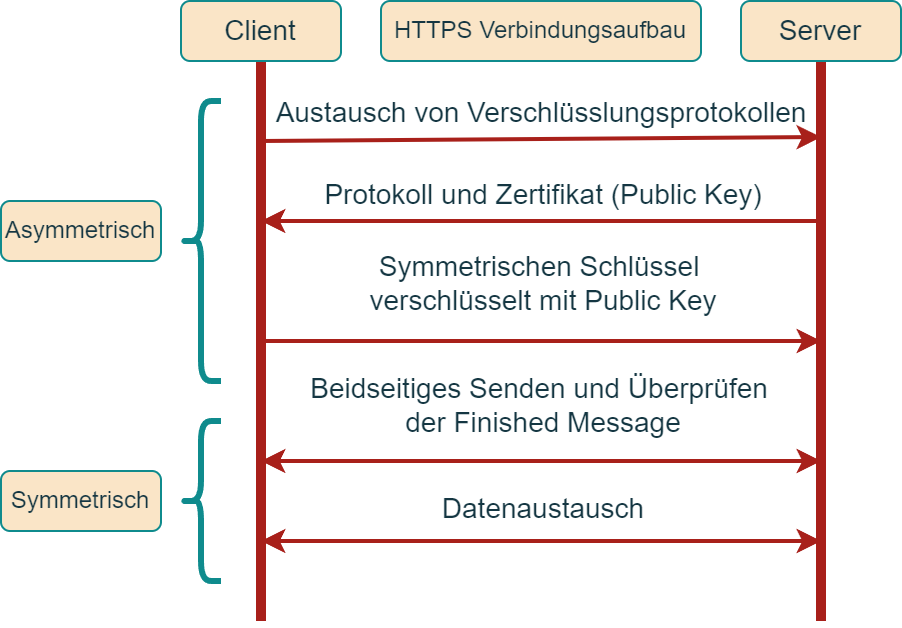
\includegraphics[width=0.45\textwidth]{sections/paul/https_verbindungsaufbau.drawio.png}
    \caption{Demonstration des HTTPS Verbindungsaufbaus}
    \label{fig:http_verbindungsaufbau}
\end{figure}
Wie in Abbildung \ref{fig:http_verbindungsaufbau} dargestellt, erfolgt der Verbindungsaufbau, indem:
\begin{enumerate}
    \item Der Client unterstützte Verschlüsselungsalgorithmen an den Server sendet.
    \item Der Server das Sicherste der unterstützten Algorithmen auswählt und das Zertifikat, welches den Public Key enthält, an den Client sendet.
    \item Folgend generiert der Client einen symmetrischen Schlüssel, welcher mit dem Public Key des Servers verschlüsselt wird.
    \item Beide überprüfen die Integrität des Schlüssels gefolgt von der tatsächlichen Kommunikation.
\end{enumerate}
\section{Funktionsweise vom RSA Algorithmus}
RSA ist ein asymmetrischer Verschlüsselungsalgorithmus.
RSA wird benötigt, um eine gesicherte Kommunikation zwischen mindestens zwei Parteien aufzubauen, da 
es andernfalls keine Möglichkeit gäbe, den Schlüssel für die symmetrische Verschlüsselung \anf{abhörsicher} zu übertragen.
Die Sicherheit beruht darauf, dass Faktorisierung von Primzahlen, da dieses ein \anf{NP\textendash Hard} Problem ist\cite{moolchad_leveraging_nodate},
also nicht in polynomieller Zeit gelöst werden kann. Die zwei Primfaktoren, welche für RSA benötigt werden, 
werden folgend mit $p$ und $q$ bezeichnet, wobei $p$ und $q$ relativ Prim zueinander sind. 
$n$ ist das Produkt dieser beiden Primfaktoren, welches bei derzeitigen RSA\textendash\ Implementierungen 
2048 Bit lang ist. Im folgenden Beispiel wird zur Nachvollziehbarkeit für $p$ und $q$ jeweils 13 und 17 gewählt, womit
$n = p \cdot q = 221$ ist. Als Zweites wird die Eulersche Phi\textendash\ Funktion benötigt, um 
\[
\phi(n) = (p-1) \cdot (q-1) = 12 \cdot 16 = 192
\]
zu berechnen. Folgend wird $e$ als Teil des Public Keys gewählt, wobei $e$ und $\phi(n)$ teilerfremd sind. In diesem 
Beispiel wird $e = 23$ gewählt. Der Public Key ist damit bereits vollständig: $(e, n) = (23, 221)$. Die letzte benötigte
Variable ist $d$, welche der erste Teil des Private Keys ist. $d$ ist das multiplikative Inverse zu $e$ modulo $\phi(n)$,
also die Zahl für die gilt:
\[
d \cdot e \equiv 1 \pmod{\phi(n)}
\]
In diesem Fall ist $d = 167$, da $167 \cdot 23 = 3841 \equiv 1 \pmod{192}$. Der Private Key ist damit $(d, n) = (167, 221)$.
Damit das Wort \anf{Dresden} tatsächlich verschlüsselt werden kann, wird dieses zu ASCII umgewandelt, wie in 
Tabelle \ref{tab:encryption_dresden} in den ersten beiden Spalten dargestellt.
% \begin{table}[h]
%     \centering
%     \begin{tabular}{|c|c|c|c|c|c|c|c|}
%         \hline
%         Buchstabe & D & r & e & s & d & e & n \\
%         \hline
%         ASCII & 68 & 114 & 101 & 115 & 100 & 101 & 110 \\
%         \hline
%     \end{tabular}
%     \caption{ASCII-Werte der Buchstaben von \anf{Dresden}}
%     \label{tab:ascii_dresden}
% \end{table}
Die Verschlüsselung erfolgt für jedes Zeichen einzeln durch:
\[
c = m^e \bmod n
\]
wobei $m$ der ASCII Code des zu verschlüsselnden Zeichens ist und $c$ der verschlüsselte Wert.
Für das Wort \anf{Dresden} ergibt sich die Verschlüsselung zu $[204, 160, 186, 123, 42, 186, 219]$, wie in Tabelle
\ref{tab:encryption_dresden} in den Spalten \anf{$m^e \bmod n$}  und \anf{$c$} dargestellt.
\begin{table}[h]
    \centering
    \begin{tabular}{|c|c|c|c|}
        \hline
        Buchstabe & m (ASCII) & $m^e \bmod n$ & $c$ \\
        \hline
        D & 68 & $68^{23} \bmod 221$ & 204 \\
        r & 114 & $114^{23} \bmod 221$ & 160 \\
        e & 101 & $101^{23} \bmod 221$ & 186 \\
        s & 115 & $115^{23} \bmod 221$ & 123 \\
        d & 100 & $100^{23} \bmod 221$ & 42 \\
        e & 101 & $101^{23} \bmod 221$ & 186 \\
        n & 110 & $110^{23} \bmod 221$ & 219 \\
        \hline
    \end{tabular}
    \caption{Verschlüsselung der einzelnen Buchstaben}
    \label{tab:encryption_dresden}
\end{table}

Die Entschlüsselung erfolgt mit dem Private Key ($d, n$) analog durch:
\[
m = c^d \bmod n
\]
wie in Tabelle \ref{tab:decryption_dresden} dargestellt ist.
\begin{table}[H]
    \centering
    \begin{tabular}{|c|c|c|c|}
        \hline
        $c$ & $c^d \bmod n$ & m (ASCII) & Buchstabe \\
        \hline
        204 & $204^{167} \bmod 221$ & 68 & D \\
        160 & $160^{167} \bmod 221$ & 114 & r \\
        186 & $186^{167} \bmod 221$ & 101 & e \\
        123 & $123^{167} \bmod 221$ & 115 & s \\
        42 & $42^{167} \bmod 221$ & 100 & d \\
        186 & $186^{167} \bmod 221$ & 101 & e \\
        219 & $219^{167} \bmod 221$ & 110 & n \\
        \hline
    \end{tabular}
    \caption{Entschlüsselung der einzelnen Buchstaben}
    \label{tab:decryption_dresden}
\end{table}
Damit ist die Nachricht \anf{Dresden} erfolgreich verschlüsselt und wieder entschlüsselt worden.



% Python output
% p=13, q=17, n=221, phi=192, e=23, d=167
% Public Key: (23, 221)
% Private Key: (167, 221)
% Encrypting message: Dresden
% D[68] -> 68**23 % 221 = 204
% r[114] -> 114**23 % 221 = 160
% e[101] -> 101**23 % 221 = 186
% s[115] -> 115**23 % 221 = 123
% d[100] -> 100**23 % 221 = 42
% e[101] -> 101**23 % 221 = 186
% n[110] -> 110**23 % 221 = 219
% Decrypting message: [204, 160, 186, 123, 42, 186, 219]
% 204^167 % 221 = 68 -> D
% 160^167 % 221 = 114 -> r
% 186^167 % 221 = 101 -> e
% 123^167 % 221 = 115 -> s
% 42^167 % 221 = 100 -> d
% 186^167 % 221 = 101 -> e
% 219^167 % 221 = 110 -> n
% Original Message: Dresden
% Encrypted Message: [204, 160, 186, 123, 42, 186, 219]
% Decrypted Message: Dresden

\section{test}
test2\\

 
\section{Der Grover-Algorithmus}
\label{sec:grover}
Der Grover-Algorithmus ist ein Quantenalgorithmus, der hilft, unstrukturierte Suchprobleme schneller zu lösen 
als klassische Methoden. Im Gegensatz zu klassischen Ansätzen, die $N$ Schritte erfordern, benötigt der 
Grover-Algorithmus nur etwa $\sqrt{N}$ Schritte, um die Lösung zu finden. Das macht ihn besonders relevant 
für die Sicherheit symmetrischer Verschlüsselungsverfahren wie AES.

\subsection{Grundprinzip}
Der Algorithmus arbeitet mit zwei Hauptschritten, die wiederholt angewendet werden:
\begin{itemize}
    \item Phasen-Inversion: Markiert die gesuchte Lösung durch Vorzeichenwechsel.
    \item Spieglung am Mittelwert: Verstärkt die Wahrscheinlichkeit, die gesuchte Lösung zu finden.
\end{itemize}

\subsubsection{Warum sind mehrere Iterationen nötig?}
Wenn die gesuchte Lösung markiert wird, wird diese zunächst nur mathematisch identifiziert, indem ihre Phase 
umgekehrt wird. Bei einer direkten Messung nach nur einem Durchlauf hätten jedoch alle Zustände noch ähnliche 
Wahrscheinlichkeiten, und die gesuchte Lösung könnte mit geringer Wahrscheinlichkeit übersehen werden. Die 
Spieglung am Mittelwert verstärkt deshalb gezielt die Amplitude der gesuchten Lösung, während die Amplituden der anderen 
Zustände verringert werden. 

Durch wiederholte Anwendung dieser beiden Schritte wird die Wahrscheinlichkeit, die richtige Lösung zu messen, 
Schritt für Schritt erhöht. Nach etwa $\sqrt{N}$ Iterationen ist diese Wahrscheinlichkeit so hoch, dass die Lösung 
mit nahezu 100\% Sicherheit gefunden wird.

\subsection{Funktionsweise}
\begin{enumerate}
    \item Initialisierung: Der Algorithmus beginnt mit einer Überlagerung aller möglichen Zustände:
        \[
        |\psi\rangle = \frac{1}{\sqrt{N}} \sum_{x=0}^{N-1} |x\rangle.
        \]

    \item Phasen-Inversion: Die gesuchte Lösung $x_{\text{target}}$ wird markiert, indem ihre Phase umkehrt wird:
        \[
        O |x\rangle = \begin{cases} 
            -|x\rangle & \text{wenn } x = x_{\text{target}}, \\
            |x\rangle & \text{sonst}.
        \end{cases}
        \]

    \item Spieglung am Mittelwert: Diese Operation verstärkt die Wahrscheinlichkeit der markierten Lösung:
        \[
        D |\psi\rangle = 2|\psi\rangle\langle\psi| - I.
        \]

    \item Wiederholung: Phasen-Inversion und Spieglung werden mehrfach angewendet (etwa $\sqrt{N}$-mal), um die 
    Wahrscheinlichkeit, die richtige Lösung zu messen, zu maximieren.
\end{enumerate}

\subsubsection{Beispiel: Suche in einer kleinen Liste}
Angenommen, wir suchen in einer Datenbank mit $N=4$ Einträgen nach der Lösung $x_{\text{target}}=2$. Die Schritte des 
Grover-Algorithmus über mehrere Iterationen lassen sich wie folgt erklären:

%%\begin{table}[H]
%%    \centering
%%    \begin{tabular}{|c|c|c|c|}
%%        \hline
%%        Iteration & Zustand & vor Diffusion & nach Diffusion \\
%%        \hline
%%        1 & $|0\rangle$ & $0.5$ & $0.25$ \\
%%        1 & $|1\rangle$ & $0.5$ & $0.25$ \\
%%       1 & $|2\rangle$ & $-0.5$ & $0.75$ \\
%%        1 & $|3\rangle$ & $0.5$ & $0.25$ \\
%%        \hline
%%        2 & $|0\rangle$ & $0.25$ & $0.125$ \\
%%        2 & $|1\rangle$ & $0.25$ & $0.125$ \\
%%        2 & $|2\rangle$ & $0.75$ & $0.875$ \\
%%        2 & $|3\rangle$ & $0.25$ & $0.125$ \\
%%        \hline
%%    \end{tabular}
%%    \caption{Amplitudenänderungen über zwei Iterationen im Grover-Algorithmus}
%%\end{table}

Nach der ersten Iteration wird die Amplitude der gesuchten Lösung ($|2\rangle$) von $-0.5$ auf $0.75$ verstärkt. 
Nach der zweiten Iteration steigt sie weiter auf $0.875$, wodurch die Wahrscheinlichkeit, diesen Zustand zu messen, deutlich zunimmt.
\\
Der Grover-Algorithmus reduziert die Sicherheit symmetrischer Verschlüsselungsverfahren wie AES. Während klassische 
Algorithmen $2^n$ Versuche benötigen, halbiert der Grover-Algorithmus diese Zahl auf $2^{n/2}$. Daher empfiehlt es sich, die 
Schlüssellängen zu verdoppeln, um quantensichere Standards zu gewährleisten \cite{grover}.


\section{Shor’s Algorithmus: Funktionsweise und mathematische Grundlage}

Shor’s Algorithmus ist ein Quantenalgorithmus, der entwickelt wurde, um 
effizient die Primfaktoren einer großen Zahl $N$ zu bestimmen. Dieses 
Problem bildet die Grundlage vieler kryptografischer Verfahren wie RSA, 
da es für klassische Computer äußerst schwierig ist, große Zahlen in 
ihre Primfaktoren zu zerlegen. Shor’s Algorithmus hingegen nutzt die 
Eigenschaften von Quantencomputern, um diese Aufgabe exponentiell 
schneller zu lösen.

\subsection{Ablauf des Algorithmus}

\begin{enumerate}
    \item \textbf{Auswahl einer Basis $a$:}  
    Zunächst wird eine Zahl $a$ gewählt, wobei $1 < a < N$ gilt. Diese 
    Basis dient als Ausgangspunkt für die nachfolgenden Berechnungen.

    \item \textbf{Periodenfindung:}  
    Der Algorithmus sucht die kleinste positive Periode $r$, sodass die 
    Kongruenzgleichung  
    \[
    a^r \mod N = 1
    \]  
    erfüllt ist. Die Periode $r$ ist der Schlüssel zur Faktorisierung von $N$.  
    \begin{itemize}
        \item Es wird sichergestellt, dass $r > 0$ ist, da eine Periode von 
        $r = 0$ keine Aussagekraft hat.
        \item Zur Bestimmung von $r$ könnte man klassisch eine Wertetabelle 
        für $r$ und die entsprechenden Werte $z = a^r \mod N$ erstellen. Da 
        diese Methode jedoch ineffizient ist, wird auf einem Quantencomputer 
        die Quanten-Fourier-Transformation (QFT) verwendet, um $r$ effizient 
        zu berechnen.
    \end{itemize}

    \item \textbf{Verwendung der Periode $r$:}  
    Sobald $r$ bekannt ist, wird geprüft:  
    \begin{itemize}
        \item Falls $r$ ungerade ist, beginnt der Algorithmus erneut mit 
        einem anderen $a$.
        \item Ist $r$ gerade, werden die Primfaktoren von $N$ mit den 
        folgenden Formeln berechnet:  
        \[
        f_1 = \text{ggT}\left(a^{r/2} - 1, N\right) \quad \text{und} \quad f_2 = \text{ggT}\left(a^{r/2} + 1, N\right).
        \]  
        Der größte gemeinsame Teiler ($\text{ggT}$) wird dabei mithilfe 
        des Euklidischen Algorithmus ermittelt.
    \end{itemize}
\end{enumerate}

\subsection{Euklidischer Algorithmus: Beispiel zur Bestimmung des ggT}

Der Euklidische Algorithmus wird verwendet, um den größten gemeinsamen 
Teiler (ggT) zweier Zahlen effizient zu bestimmen. Anhand des Beispiels 
$N_1 = 132$ und $N_2 = 28$ wird der Algorithmus wie folgt angewendet:

\begin{enumerate}
    \item \textbf{Schritt 1:}  
    Teile die größere Zahl durch die kleinere und bestimme den Rest:  
    \[
    132 \div 28 = 4 \, \text{Rest} \, 20 \quad \Rightarrow \quad 132 = 4 \cdot 28 + 20.
    \]

    \item \textbf{Schritt 2:}  
    Die vorherige Divisorzahl $28$ wird der neue Dividend, und der Rest $20$ wird der neue Divisor:  
    \[
    28 \div 20 = 1 \, \text{Rest} \, 8 \quad \Rightarrow \quad 28 = 1 \cdot 20 + 8.
    \]

    \item \textbf{Schritt 3:}  
    Wiederhole den Vorgang, bis der Rest $0$ wird:  
    \[
    20 \div 8 = 2 \, \text{Rest} \, 4 \quad \Rightarrow \quad 20 = 2 \cdot 8 + 4,
    \]  
    \[
    8 \div 4 = 2 \, \text{Rest} \, 0 \quad \Rightarrow \quad 8 = 2 \cdot 4 + 0.
    \]
\end{enumerate}

Der letzte Divisor, bevor der Rest $0$ wird, ist der gesuchte größte gemeinsame Teiler:  
\[
\text{ggT}(132, 28) = 4.
\]

\subsection{Quantenteil des Shor Algorithmus}

% \section{Forschungsfrage}
% Die Studie zielt darauf ab, die technischen und organisatorischen Auswirkungen 
% von Quantencomputern auf die IT-Sicherheit zu untersuchen, mit besonderem Fokus 
% auf kryptografische Verfahren. Dabei verfolgt sie einen Mixed-Methods-Ansatz, 
% der sowohl technische Analysen als auch qualitative Befragungen kombiniert, um 
% ein umfassendes Verständnis der Risiken und Handlungsoptionen zu gewinnen.

\section{Methodisches Vorgehen}

Die Untersuchung folgt einem Mixed-Methods-Ansatz, der sowohl technische als auch organisatorische Aspekte berücksichtigt. 
Im Rahmen der technischen Analyse (FF1) werden zwei klassische Verschlüsselungsalgorithmen, RSA und AES, auf 
konventionellen Systemen hinsichtlich ihrer Verschlüsselungs- und Entschlüsselungszeiten analysiert. Diese 
Tests berücksichtigen unterschiedliche Schlüssellängen und Datenmengen, um die Effizienz der Algorithmen unter 
variierenden Bedingungen zu bewerten, welche in Tabelle \ref{tab:schluessel_datenmengen} dargestellt sind. 
\begin{table}[ht]
    \centering
    \begin{tabularx}{0.45 \textwidth}{X X X}
    \hline
    \textbf{Algorithmus} & \textbf{Schlüssellängen} & \textbf{Datenmengen} \\
    \hline
    \text{RSA} & 1024, 2048, 4096, 8129 \text{ Bit} & 117, 245, 373, 501, 1013 \text{Byte}\\
    \hline
    \text{AES} & 128, 192, 256 \text{ Bit} & 1 \text{ KB}, 10 \text{ KB}, 100 \text{ KB}, 1 \text{ MB}, 5 \text{ MB}\\
    \hline
    \end{tabularx}
    \caption{Zu testende Schlüssellängen und Datenmengen}
    \label{tab:schluessel_datenmengen}
\end{table}
Die sehr spezifischen Datenmengen bei RSA beziehen sich auf die maximale Datenmenge pro Schlüssellaenge. 
Am Beispiel von 4096 Bit Verschlüsselung, würde diese zu Bytes umgerechnet werden. Diesen 
werden folgend 11 Bytes (konstant bei allen Schlüssellängen) abgezogen, da diese als sogenanntes Padding dienen. Damit ergibt sich $4096/8 - 11 = 501$. 
Bei AES beziehen sich die Datenmengen auf gängige zu Größen, welche bei HTTPS übertragen werden, da hierbei AES mit RSA kombiniert wird 
(Abbildung \ref{fig:http_verbindungsaufbau}).
Die Ergebnisse werden mit dokumentierten Benchmarks von Quantenalgorithmen 
wie Shor's und Grover's Algorithmus verglichen. Ergänzend werden analytische Methoden genutzt, um die theoretische 
Effizienz dieser Quantenalgorithmen zu modellieren. Diese Berechnungen basieren auf dokumentierten Benchmarks 
aktueller Quantencomputer und Zeitkomplexitätsmodellen, um kritische Schlüssellängen zu identifizieren, bei denen 
bestehende Verschlüsselungsverfahren potenziell gefährdet sind.

Die organisatorische Analyse (FF2) stützt sich auf qualitative Befragungen von IT-Sicherheitsverantwortlichen. 
In leitfadengestützten Interviews werden Einschätzungen zu den Risiken durch Quantencomputer 
sowie zur Dringlichkeit und Machbarkeit neuer kryptografischer Standards erhoben. Die Antworten werden thematisch 
analysiert, um zentrale Herausforderungen und Handlungsstrategien zu identifizieren. Ein besonderer Fokus liegt dabei 
auf präventiven Maßnahmen und ihrer zeitlichen Priorisierung. Beispielhafte Interviewfragen lauten:

\begin{itemize}
    \item „Wie schätzen Sie die Gefahr ein, die Quantencomputer für aktuelle Verschlüsselungsverfahren darstellen?“
    \item „Welche Maßnahmen halten Sie für besonders wichtig, um sich gegen diese Risiken abzusichern?“
    \item „Wie dringend ist Ihrer Meinung nach die Einführung von Post-Quanten-Kryptografie?“
    \item „Welche Herausforderungen sehen Sie bei der Umsetzung solcher Sicherheitsstandards?“
    \item „Gibt es Branchen, die Ihrer Meinung nach besonders von der Entwicklung der Quantencomputer betroffen sein werden?“
\end{itemize}

Die Ergebnisse beider Analyseschritte werden integriert, um ein umfassendes Verständnis der Risiken und 
Handlungsoptionen zu ermöglichen. Technische Erkenntnisse und Experteneinschätzungen werden kombiniert, um 
praxisorientierte Empfehlungen für Unternehmen zur Vorbereitung auf die Ära des Quantencomputings abzuleiten.\\

Das erwartete Ergebnis ist eine klare Einschätzung der Auswirkungen von Quantencomputern 
auf klassische Verschlüsselungsverfahren und die Identifikation von Risiken sowie 
Handlungsmöglichkeiten für Unternehmen. Durch das Benchmarking wird erwartet, dass RSA auf klassischen Computern nahezu 
unbrechbar ist, jedoch auf Quantencomputern exponentiell schneller gebrochen werden kann. 
Bei AES wird erwartet, dass der Algorithmus auf klassischen Computern 
eine hohe Sicherheit bietet, während Grover's Algorithmus die Effizienz 
der Entschlüsselung ungefähr halbiert, jedoch nicht exponentiell verringert.
Die Ergebnisse sollen praxisnahe Empfehlungen 
für den Übergang zu post-quanten-kryptografischen Standards liefern.

\section{Fazit}
Die Analyse der Auswirkungen von Quantencomputern auf Verschlüsselungsalgorithmen
zeigt deutliche Bedrohungen auf die IT-Sicherheit. Insbesondere asymmetrische 
Verschlüsselungsverfahren wie RSA sind durch Shore's Algorithmus gefährdet. 
Der Grund liegt in der Fähigkeit von Quantencomputern, mit diesem Algorithmus
die Primfaktoren einer Zahl, wie zum Beispiel ein 2048 Bit RSA Schlüssel, 
effizient zu berechnen, wie in Sektion \ref{sec:shor} beschrieben wurde.\\
Auch AES ist durch den Grover-Algorithmus (siehe Sektion \ref{sec:grover}) bedroht, welcher die Rechenzeit 
halbiert, um den Schlüssel zu finden. Allerdings bietet dieser 
nicht wie Shore's Algorithmus eine exponentiell schnellere Berechnung und ist somit
grundlegend noch als sicher zu betrachten.\\
Bezüglich der ersten Forschungsfrage lässt sich festhalten, dass symmetrische 
Verschlüsselungsalgorithmen wie AES weniger stark betroffen sind als 
asymmetrische Verfahren. Während RSA durch Shor's Algorithmus praktisch 
gebrochen werden kann (siehe Sektion \ref{sec:shor}), bietet AES,
wie in Sektion \ref{sec:aes} dargestellt wurde, durch seine komplexe Struktur aus SubBytes, 
ShiftRows, MixColumns und der Rundenschlüssel auch gegenüber Quantencomputern 
noch Sicherheit, wenn auch mit erhöhten Anforderungen an die Schlüssellänge.\\
Die zweite Forschungsfrage hinsichtlich \anf{Store now, decrypt later-Angriffen}
zeigt die Dringlichkeit des Problems: Selbst wenn 
aktuelle Quantencomputer noch nicht leistungsfähig 
genug sind, sollten Unternehmen und Regierungen, bereits möglichst zeitnah 
Maßnahmen ergreifen, da verschlüsselte Daten gespeichert 
und später entschlüsselt werden könnten, wie in Sektion 
\ref{sec:quantencomputer} dargestellt wurde.\\

\subsection{Ausblick}
Die Forschung im Bereich der Quantenkryptographie stellt eine erhebliche 
Herausforderung für die IT-Sicherheit dar, da RSA praktisch gebrochen werden 
kann. Auch andere weit verbreitete Alternative Algorithmen wie \anf{Elliptic Curve \textendash ED25519},
sind durch den Shor's Algorithmus gefährdet. Dies betrifft sowol direkt als auch indirekt symmetrische
Verschlüsselungsalgorithmen, da diese oft in Kombination 
mit asymmetrischen Verfahren, wie in Abbildung \ref{fig:http_verbindungsaufbau} dargestellt, 
verwendet werden. Das ist vor allem für die Kommunikationstechnik von Relevanz, da nun
Verbindungen kompromittiert werden können, da symmetrische Schlüssel mithilfe
von asymmetrischen Verfahren ausgetauscht werden.\\



\newpage

%%
%% The next two lines define the bibliography style to be used, and
%% the bibliography file.
\bibliographystyle{ACM-Reference-Format}
\bibliography{sample-base}


%%
%% If your work has an appendix, this is the place to put it.
\appendix

\end{document}
\endinput
%%
%% End of file `sample-sigconf-authordraft.tex'.
